\chapter{解析方法}
ハイスピードカメラを用いて落下球が落下する様子をbmp形式の連続画像として撮影するとFig.\ref{fig:expPhoto}(a) に示すように落下球以外にも電磁石や水槽壁面が存在する.この画像から,落下球を検出するためにHough変換を用いた.しかし,Hough変換は任意の幾何形状を表す円に対して特徴点に対して一定数以上通る円を検出する変換手法であるため,球の輪郭が必要となる.本実験では落下球の輪郭を描く方法として背景処理とSobel filterを用いた.
\section{背景処理とSobel filter}
Hough変換を行う前処理として,背景処理とSobel filterの処理を行った.撮影した連続画像に背景処理を行うとFig.\ref{fig:expPhoto}(b) に示すようになった.背景処理では,画像輝度値の平均値をとり,それぞれの画像との差分を取り,それぞれの画像における差分を明確にした.続いて,背景処理を行った画像へSobel filterの処理を行った.Sobel filterとは,輪郭抽出を行うフィルタ処理である.具体的な処理として,ある任意の画素を中心とした9つの輝度値に対し,

\begin{figure}[h]
    \centering
    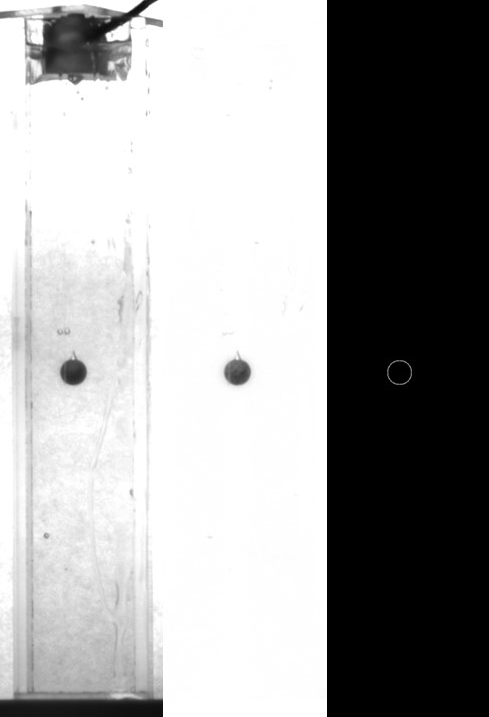
\includegraphics[scale=0.8,clip]{3-Analysis/exp-img.png}
    \caption{(a) Original image, (b) Image used by background processing and, (c) Image used by Sobel filter.}
    \label{fig:expPhoto}
\end{figure}

\section{Hough変換による円の検出}
背景処理とSobel filter処理を行った画像内から鋼球の検出を行うために,Hough変換による円検出を用いた.検出手順は,以下に示す通りである.円は中心座標と半径により一意に定まる.このことより,円の中心座標 ($x_c$, $y_c$) ,半径r による1つの円D ($x_c$, $y_c$, r) に関して考える.
